\documentclass[notes,11pt, aspectratio=169]{beamer}

\usepackage{pgfpages}
\setbeameroption{hide notes} % Only slide

\usepackage{array}
\usepackage{tikz}
\usepackage{verbatim}
\setbeamertemplate{note page}{\pagecolor{gray!5}\insertnote}
\usetikzlibrary{positioning}
\usetikzlibrary{snakes}
\usetikzlibrary{calc}
\usetikzlibrary{arrows}
\usetikzlibrary{decorations.markings}
\usetikzlibrary{shapes.misc}
\usetikzlibrary{matrix,shapes,arrows,fit,tikzmark}
\usepackage{amsmath}
\usepackage{mathpazo}
\usepackage{hyperref}
\usepackage{lipsum}
\usepackage{multimedia}
\usepackage{graphicx}
\usepackage{multirow}
\usepackage{dcolumn}
\usepackage{bbm}
\newcolumntype{d}[0]{D{.}{.}{5}}

\usepackage{changepage}
\usepackage{appendixnumberbeamer}

\usepackage[space]{grffile}
\usepackage{booktabs}

% Colors
\definecolor{blue}{RGB}{0,114,178}
\definecolor{red}{RGB}{213,94,0}
\definecolor{yellow}{RGB}{240,228,66}
\definecolor{green}{RGB}{0,158,115}
\definecolor{solutionbg}{RGB}{240,248,240}
\definecolor{solutionframe}{RGB}{0,158,115}

% Solution box environment for worked answers
\usepackage{tcolorbox}
\newtcolorbox{solutionbox}[1][]{
  enhanced,
  colback=solutionbg,
  colframe=solutionframe,
  boxrule=0pt,
  leftrule=3pt,
  arc=0pt,
  left=8pt,
  right=8pt,
  top=6pt,
  bottom=6pt,
  fonttitle=\bfseries,
  title={#1},
  attach boxed title to top left={yshift=-2mm, xshift=5mm},
  boxed title style={colback=solutionframe, colframe=solutionframe, size=small, arc=2pt}
}

\hypersetup{
  colorlinks=false,
  linkbordercolor = {white},
  linkcolor = {blue}
}

\definecolor{MyBackground}{RGB}{255,253,218}

\newenvironment{transitionframe}{
  \setbeamercolor{background canvas}{bg=white}
  \begin{frame}}{
    \end{frame}
}

\setbeamercolor{frametitle}{fg=blue}
\setbeamercolor{title}{fg=black}
\setbeamertemplate{footline}[frame number]
\setbeamertemplate{navigation symbols}{}
\setbeamertemplate{itemize items}{-}
\setbeamercolor{itemize item}{fg=blue}
\setbeamercolor{itemize subitem}{fg=blue}
\setbeamercolor{enumerate item}{fg=blue}
\setbeamercolor{enumerate subitem}{fg=blue}
\setbeamercolor{button}{bg=MyBackground,fg=blue,}

\setbeamercolor{section in toc}{fg=blue}
\setbeamercolor{subsection in toc}{fg=red}
\setbeamersize{text margin left=1em,text margin right=1em}

\newenvironment{wideitemize}{\itemize\addtolength{\itemsep}{10pt}}{\enditemize}
\newenvironment{wideenumerate}{\enumerate\addtolength{\itemsep}{10pt}}{\endenumerate}

\title[]{\textcolor{blue}{ECN 594: Entry and Market Structure}}
\author[PGP]{}
\institute[FRBNY]{\small{\begin{tabular}{c c c}
Nicholas Vreugdenhil \\
\end{tabular}}}
\date{\today}

\begin{document}

% Title Slide
\begin{frame}
\maketitle
  \centering
\end{frame}

\begin{frame}{Plan}
  \begin{wideenumerate}
    \item \textbf{What determines market structure?}
    \item Free entry condition
    \item Entry with Cournot: worked example
    \item Entry barriers
    \item Entry deterrence strategies
    \item Sequential game analysis (from ECN 532)
  \end{wideenumerate}
\end{frame}

%%%%%%%%%%%%%%%%%%%%%%%%%%%%%%%%%%%%%%%%%%%%%%%%%%%%%%%%%%%%%
% ENTRY AND MARKET STRUCTURE
%%%%%%%%%%%%%%%%%%%%%%%%%%%%%%%%%%%%%%%%%%%%%%%%%%%%%%%%%%%%%

\begin{frame}{What determines market structure?}
	\begin{wideitemize}
		\item Why do some industries have many firms (restaurants) and others few (aircraft)?
		\item \textbf{Key factors:}
		\begin{wideenumerate}
			\vspace{5pt}
			\item Fixed costs of entry
			\item Market size (demand)
			\item Nature of competition
			\item Entry barriers
		\end{wideenumerate}
		\item Today: focus on entry decisions and barriers
	\end{wideitemize}
\end{frame}

\begin{frame}{Plan}
  \begin{wideenumerate}
    \item What determines market structure?
    \item \textbf{Free entry condition}
    \item Entry with Cournot: worked example
    \item Entry barriers
    \item Entry deterrence strategies
    \item Sequential game analysis (from ECN 532)
  \end{wideenumerate}
\end{frame}

\begin{frame}{Free entry condition}
	\begin{wideitemize}
		\item Suppose entry requires fixed cost $F$
		\item \textbf{Entry decision:} Enter if $\pi(N) > F$
		\begin{wideitemize}
			\vspace{5pt}
			\item $\pi(N)$ = profit when $N$ firms in market
		\end{wideitemize}
		\item \textbf{Free entry equilibrium:} Number of firms $N^*$ such that:
		\begin{align*}
			\pi(N^*) \geq F > \pi(N^* + 1)
		\end{align*}
		\item \textbf{Intuition:}
		\begin{wideitemize}
			\vspace{5pt}
			\item Current firms earn enough to cover $F$
			\item One more firm would push profits below $F$
		\end{wideitemize}
	\end{wideitemize}
\end{frame}

\begin{frame}{Entry reduces profits}
	\begin{wideitemize}
		\item As $N$ increases:
		\begin{wideitemize}
			\vspace{5pt}
			\item Competition intensifies
			\item Prices fall
			\item Each firm's profit falls
		\end{wideitemize}
		\item $\pi(N)$ is decreasing in $N$
		\item Eventually: $\pi(N) < F$ and entry stops
	\end{wideitemize}
\end{frame}

\begin{frame}{Entry reduces profits: graphical}
	\begin{center}
		\begin{tikzpicture}[scale=0.8]
			\draw[->] (0,0) -- (8,0) node[right] {$N$};
			\draw[->] (0,0) -- (0,5) node[above] {$\pi$};

			% Profit curve
			\draw[thick, blue, domain=1:7, smooth] plot (\x, {4/(\x*\x/4 + 0.5)});
			\node[blue, right] at (7,0.8) {$\pi(N)$};

			% Fixed cost line
			\draw[dashed, red] (0,1.5) -- (8,1.5) node[right] {$F$};

			% Equilibrium
			\draw[dashed] (3,0) -- (3,1.5);
			\node[below] at (3,0) {$N^*$};

			% Labels
			\node[left] at (0,1.5) {$F$};
		\end{tikzpicture}
	\end{center}
	\begin{wideitemize}
		\item Entry continues until $\pi(N) = F$
		\item $N^*$ = equilibrium number of firms
	\end{wideitemize}
\end{frame}

\begin{frame}{Comparative statics of entry}
	\begin{wideitemize}
		\item \textbf{How does $N^*$ change when:}
		\item Market size $\uparrow$: $N^* \uparrow$ (more room for firms)
		\item Fixed cost $F \uparrow$: $N^* \downarrow$ (harder to cover costs)
		\item Marginal cost $c \uparrow$: $N^* \downarrow$ (lower profit margins)
		\item Competition intensity $\uparrow$: $N^* \downarrow$ (profits lower for any $N$)
		\item \textbf{Prediction:} Large markets with low entry costs have many small firms
	\end{wideitemize}
\end{frame}

\begin{frame}{Practice: Free entry}
	\begin{wideitemize}
		\item \textbf{True, False, or NEI:}
		\item (a) In a free entry equilibrium, all firms earn zero profit.
		\item (b) Higher fixed costs lead to more concentrated industries.
		\item (c) Under Bertrand competition with homogeneous products, free entry leads to the same number of firms as Cournot.
	\end{wideitemize}
	\vspace{10pt}
	\centering
	\textit{Take 2 minutes.}
\end{frame}

\begin{frame}{Practice: Free entry (solution)}
	\begin{solutionbox}[Answers]
		\begin{wideitemize}
			\item \textbf{(a) FALSE.} Firms earn $\pi(N^*) \geq F$. Integer constraint means they may earn more than $F$.
			\item \textbf{(b) TRUE.} Higher $F$ means fewer firms can cover their fixed costs. Industries are more concentrated.
			\item \textbf{(c) FALSE.} Under Bertrand with homogeneous products, $P = MC$ even with 2 firms. More entry doesn't change profits---1 firm would be monopoly, 2+ gives $P = MC$.
		\end{wideitemize}
	\end{solutionbox}
\end{frame}

\begin{frame}{Plan}
  \begin{wideenumerate}
    \item What determines market structure?
    \item Free entry condition
    \item \textbf{Entry with Cournot: worked example}
    \item Entry barriers
    \item Entry deterrence strategies
    \item Sequential game analysis (from ECN 532)
  \end{wideenumerate}
\end{frame}

\begin{frame}{Entry with Cournot: setup}
	\begin{wideitemize}
		\item Inverse demand: $P = a - bQ$
		\item $N$ symmetric firms, each with $MC = c$
		\item Fixed cost of entry: $F$
		\item Cournot equilibrium with $N$ firms:
		\begin{align*}
			q_i^* &= \frac{a - c}{b(N + 1)} \\
			P^* &= \frac{a + Nc}{N + 1} \\
			\pi_i^* &= \frac{(a - c)^2}{b(N + 1)^2}
		\end{align*}
	\end{wideitemize}
\end{frame}

\begin{frame}{Worked example: Entry with Cournot}
	\begin{wideitemize}
		\item \textbf{Question:} $P = 100 - Q$, $c = 20$, $F = 100$.
		\item How many firms will enter in equilibrium?
	\end{wideitemize}
	\vspace{15pt}
	\centering
	\textit{Take 5 minutes.}
\end{frame}

\begin{frame}{Worked example: Entry (solution)}
	\begin{solutionbox}[Solution]
		\begin{wideitemize}
			\item With $a = 100$, $b = 1$, $c = 20$:
			\begin{align*}
				\pi(N) = \frac{(100 - 20)^2}{(N + 1)^2} = \frac{6400}{(N + 1)^2}
			\end{align*}
			\item Check different values of $N$:
			\begin{center}
				\begin{tabular}{|c|c|c|}
					\hline
					$N$ & $\pi(N)$ & Enter? \\
					\hline
					1 & $6400/4 = 1600$ & Yes ($> 100$) \\
					2 & $6400/9 = 711$ & Yes \\
					3 & $6400/16 = 400$ & Yes \\
					5 & $6400/36 = 178$ & Yes \\
					7 & $6400/64 = 100$ & Indifferent \\
					8 & $6400/81 = 79$ & No ($< 100$) \\
					\hline
				\end{tabular}
			\end{center}
			\item \textbf{Answer:} $N^* = 7$ firms enter
		\end{wideitemize}
	\end{solutionbox}
\end{frame}

\begin{frame}{Fixed costs and natural monopoly}
	\begin{wideitemize}
		\item When $F$ is very high relative to demand:
		\begin{wideitemize}
			\vspace{5pt}
			\item Only one firm can profitably operate
			\item \textbf{Natural monopoly}
		\end{wideitemize}
		\item \textbf{Examples:}
		\begin{wideitemize}
			\vspace{5pt}
			\item Utilities (water, electricity distribution)
			\item Railroad tracks
			\item Cable infrastructure
		\end{wideitemize}
		\item Average cost is declining over relevant range
		\item One firm can serve entire market more cheaply than multiple firms
	\end{wideitemize}
\end{frame}

\begin{frame}{Practice: Market structure}
	\begin{wideitemize}
		\item \textbf{Question:} Two industries with same demand $P = 100 - Q$.
		\item Industry A: $F_A = 200$, $c_A = 10$ (Cournot)
		\item Industry B: $F_B = 50$, $c_B = 30$ (Cournot)
		\item Which industry will have more firms in equilibrium?
	\end{wideitemize}
	\vspace{10pt}
	\centering
	\textit{Take 3 minutes.}
\end{frame}

\begin{frame}{Practice: Market structure (solution)}
	\begin{solutionbox}[Solution]
		\begin{wideitemize}
			\item Industry A: $\pi_A(N) = \frac{(100-10)^2}{(N+1)^2} = \frac{8100}{(N+1)^2}$
			\begin{wideitemize}
				\vspace{3pt}
				\item $N=5$: $\pi = 225 > 200$ (Enter)
				\item $N=6$: $\pi = 165 < 200$ (No)
				\item $\Rightarrow N^*_A = 5$
			\end{wideitemize}
			\item Industry B: $\pi_B(N) = \frac{(100-30)^2}{(N+1)^2} = \frac{4900}{(N+1)^2}$
			\begin{wideitemize}
				\vspace{3pt}
				\item $N=8$: $\pi = 60 > 50$ (Enter)
				\item $N=9$: $\pi = 49 < 50$ (No)
				\item $\Rightarrow N^*_B = 8$
			\end{wideitemize}
			\item Industry B has more firms despite higher MC (lower $F$ dominates)
		\end{wideitemize}
	\end{solutionbox}
\end{frame}

\begin{frame}{Excess entry theorem (brief)}
	\begin{wideitemize}
		\item Free entry may produce ``too many'' firms
		\item \textbf{Why?} Each entrant ignores:
		\begin{wideenumerate}
			\vspace{5pt}
			\item Business-stealing effect: takes customers from incumbents
			\item Consumer surplus: captured by entrant, not new value created
		\end{wideenumerate}
		\item Private incentive to enter $>$ social incentive
		\item \textbf{Result:} Free entry equilibrium can have more firms than socially optimal
		\item Caveat: depends on model specifics
	\end{wideitemize}
\end{frame}

%%%%%%%%%%%%%%%%%%%%%%%%%%%%%%%%%%%%%%%%%%%%%%%%%%%%%%%%%%%%%
% ENTRY DETERRENCE
%%%%%%%%%%%%%%%%%%%%%%%%%%%%%%%%%%%%%%%%%%%%%%%%%%%%%%%%%%%%%

\begin{frame}{Plan}
  \begin{wideenumerate}
    \item What determines market structure?
    \item Free entry condition
    \item Entry with Cournot: worked example
    \item \textbf{Entry barriers}
    \item Entry deterrence strategies
    \item Sequential game analysis (from ECN 532)
  \end{wideenumerate}
\end{frame}

\begin{frame}{Entry barriers}
	\begin{wideitemize}
		\item \textbf{Structural barriers:} inherent to industry
		\begin{wideitemize}
			\vspace{5pt}
			\item Economies of scale (high $F$)
			\item Capital requirements
			\item Patents and intellectual property
			\item Network effects
		\end{wideitemize}
		\item \textbf{Strategic barriers:} created by incumbents
		\begin{wideitemize}
			\vspace{5pt}
			\item Limit pricing
			\item Capacity commitment
			\item Product proliferation
			\item Long-term contracts with customers
		\end{wideitemize}
	\end{wideitemize}
\end{frame}

\begin{frame}{Plan}
  \begin{wideenumerate}
    \item What determines market structure?
    \item Free entry condition
    \item Entry with Cournot: worked example
    \item Entry barriers
    \item \textbf{Entry deterrence strategies}
    \item Sequential game analysis (from ECN 532)
  \end{wideenumerate}
\end{frame}

\begin{frame}{Entry deterrence: the key question}
	\begin{wideitemize}
		\item Can an incumbent prevent entry?
		\item \textbf{The credibility problem:}
		\begin{wideitemize}
			\vspace{5pt}
			\item Incumbent threatens to ``fight'' if entry occurs
			\item But is this threat credible?
			\item Once entry happens, fighting may hurt the incumbent too
		\end{wideitemize}
		\item \textbf{From ECN 532:} Need subgame perfect equilibrium (SPE)
		\begin{wideitemize}
			\vspace{5pt}
			\item Check what incumbent would actually do if entry occurs
			\item Non-credible threats are ignored
		\end{wideitemize}
	\end{wideitemize}
\end{frame}

\begin{frame}{Entry game: basic structure}
	\begin{center}
		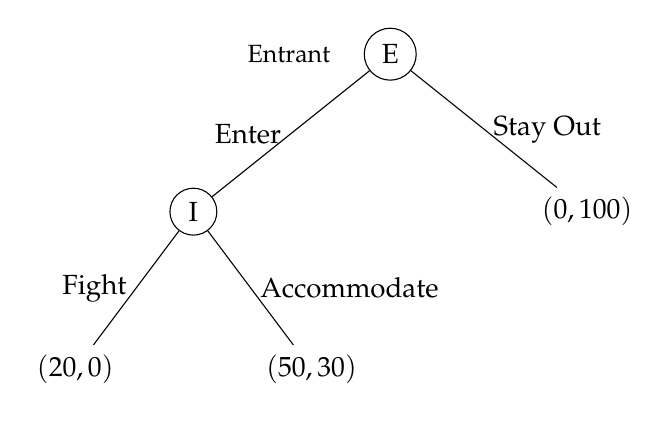
\begin{tikzpicture}[
			level 1/.style={sibling distance=5cm, level distance=2cm},
			level 2/.style={sibling distance=3cm, level distance=2cm}
		]
			\node[circle, draw] (E) {E}
			child {
				node[circle, draw] (I) {I}
				child {node {$(20, 0)$} edge from parent node[left] {Fight}}
				child {node {$(50, 30)$} edge from parent node[right] {Accommodate}}
				edge from parent node[left] {Enter}
			}
			child {
				node {$(0, 100)$}
				edge from parent node[right] {Stay Out}
			};
			\node[left=0.3cm of E] {\small Entrant};
		\end{tikzpicture}
	\end{center}
	\begin{wideitemize}
		\item Payoffs: (Entrant, Incumbent)
		\item If I would Accommodate, threat to Fight is not credible
	\end{wideitemize}
\end{frame}

\begin{frame}{Finding the SPE}
	\begin{wideitemize}
		\item \textbf{Step 1: Incumbent's decision (if entry occurs)}
		\begin{wideitemize}
			\vspace{5pt}
			\item Fight: $\pi_I = 0$
			\item Accommodate: $\pi_I = 30$
			\item $\Rightarrow$ Incumbent accommodates
		\end{wideitemize}
		\item \textbf{Step 2: Entrant's decision (knowing I will accommodate)}
		\begin{wideitemize}
			\vspace{5pt}
			\item Enter: $\pi_E = 50$
			\item Stay Out: $\pi_E = 0$
			\item $\Rightarrow$ Entrant enters
		\end{wideitemize}
		\item \textbf{SPE:} (Enter, Accommodate) with payoffs $(50, 30)$
		\item Entry not deterred because threat wasn't credible
	\end{wideitemize}
\end{frame}

\begin{frame}{Limit pricing}
	\begin{wideitemize}
		\item Incumbent sets price low enough that entry is unprofitable
		\item \textbf{Idea:} If $P$ is low, post-entry profits are low
		\item \textbf{Problem:} Why would incumbent maintain low $P$ after entry?
		\begin{wideitemize}
			\vspace{5pt}
			\item If entrant enters anyway, incumbent may prefer to accommodate
			\item Threat to keep $P$ low may not be credible
		\end{wideitemize}
		\item Works better if low $P$ is a commitment device
		\item Or if low $P$ signals low costs
	\end{wideitemize}
\end{frame}

\begin{frame}{Capacity commitment}
	\begin{wideitemize}
		\item Incumbent builds excess capacity before entry decision
		\item \textbf{Why it works:}
		\begin{wideitemize}
			\vspace{5pt}
			\item Capacity is a sunk cost
			\item With excess capacity, incumbent's marginal cost is low
			\item Post-entry, incumbent will produce more (use the capacity)
			\item Entrant anticipates this $\rightarrow$ lower post-entry profits
		\end{wideitemize}
		\item \textbf{Key insight:} Capacity makes ``fight'' credible
		\item Building capacity is a commitment device
	\end{wideitemize}
\end{frame}

\begin{frame}{Plan}
  \begin{wideenumerate}
    \item What determines market structure?
    \item Free entry condition
    \item Entry with Cournot: worked example
    \item Entry barriers
    \item Entry deterrence strategies
    \item \textbf{Sequential game analysis (from ECN 532)}
  \end{wideenumerate}
\end{frame}

\begin{frame}{Entry deterrence game: structure}
	\begin{wideitemize}
		\item \textbf{Stage 1:} Incumbent chooses capacity $K$
		\item \textbf{Stage 2:} Entrant observes $K$ and decides: Enter or Stay Out
		\item \textbf{Stage 3:} If entry, firms compete (Cournot or Bertrand)
		\item Solve by \textbf{backward induction} (from ECN 532):
		\begin{wideenumerate}
			\vspace{5pt}
			\item Find post-entry equilibrium profits given $K$
			\item Determine when entrant enters
			\item Find incumbent's optimal $K$
		\end{wideenumerate}
	\end{wideitemize}
\end{frame}

\begin{frame}{Worked example: Entry deterrence}
	\begin{wideitemize}
		\item \textbf{Setup:}
		\item Inverse demand: $P = 100 - Q$
		\item Incumbent has capacity $K$ (sunk), $MC = 0$ up to $K$
		\item Entrant has $MC = 20$, fixed cost $F = 200$
		\item If entry: Cournot competition
		\item \textbf{Question:} What $K$ deters entry?
	\end{wideitemize}
	\vspace{10pt}
	\centering
	\textit{Take 5 minutes to set up the backward induction.}
\end{frame}

\begin{frame}{Worked example: Entry deterrence (solution 1)}
	\begin{solutionbox}[Solution]
		\begin{wideitemize}
			\item \textbf{Step 1: Post-entry equilibrium}
			\item Incumbent produces $q_I \leq K$ at $MC = 0$
			\item Entrant FOC: $100 - 2q_E - q_I - 20 = 0 \Rightarrow q_E = 40 - q_I/2$
			\item If $K$ is large, incumbent produces $q_I = K$
			\item Entrant produces: $q_E = 40 - K/2$
			\item Price: $P = 100 - K - (40 - K/2) = 60 - K/2$
			\item Entrant profit: $\pi_E = (60 - K/2 - 20)(40 - K/2) = (40 - K/2)^2$
		\end{wideitemize}
	\end{solutionbox}
\end{frame}

\begin{frame}{Worked example: Entry deterrence (solution 2)}
	\begin{solutionbox}[Solution]
		\begin{wideitemize}
			\item \textbf{Step 2: Entry decision}
			\item Entrant enters if: $\pi_E - F > 0$
			\begin{align*}
				(40 - K/2)^2 > 200
			\end{align*}
			\item Entry occurs if: $40 - K/2 > \sqrt{200} \approx 14.1$
			\item Entry is deterred if: $K \geq 2(40 - 14.1) = 51.8$
			\item \textbf{Step 3: Incumbent's choice}
			\item If deterrence is profitable: Set $K \geq 52$
			\item Compare: monopoly profits with $K = 52$ vs accommodation
		\end{wideitemize}
	\end{solutionbox}
\end{frame}

\begin{frame}{When is deterrence profitable?}
	\begin{wideitemize}
		\item Incumbent compares:
		\begin{wideenumerate}
			\vspace{5pt}
			\item \textbf{Deter:} Monopoly profits minus cost of excess capacity
			\item \textbf{Accommodate:} Duopoly profits
		\end{wideenumerate}
		\item Deterrence is profitable when:
		\begin{wideitemize}
			\vspace{5pt}
			\item Cost of deterrence (excess capacity) is low
			\item Post-entry competition is intense
			\item Monopoly profits are high
		\end{wideitemize}
		\item Sometimes: accommodation is better (``puppy dog'' strategy)
	\end{wideitemize}
\end{frame}

\begin{frame}{Fudenberg-Tirole taxonomy}
	\begin{center}
	\begin{tabular}{|l|c|c|}
		\hline
		& \textbf{Deter} & \textbf{Accommodate} \\
		\hline
		\textbf{Tough} & Top Dog & Lean \& Hungry \\
		& (Overinvest) & (Underinvest) \\
		\hline
		\textbf{Soft} & Puppy Dog & Fat Cat \\
		& (Underinvest) & (Overinvest) \\
		\hline
	\end{tabular}
	\end{center}
	\vspace{5pt}
	\begin{wideitemize}
		\item ``Tough'' = investment makes incumbent more aggressive
		\item ``Soft'' = investment makes incumbent less aggressive
		\item Optimal strategy depends on competition type!
	\end{wideitemize}
\end{frame}

\begin{frame}{Practice: Entry deterrence}
	\begin{wideitemize}
		\item \textbf{True, False, or NEI:}
		\item (a) An incumbent should always try to deter entry.
		\item (b) Building excess capacity is always a credible deterrent.
		\item (c) Limit pricing works better when entrant believes incumbent has low costs.
	\end{wideitemize}
	\vspace{10pt}
	\centering
	\textit{Take 2 minutes.}
\end{frame}

\begin{frame}{Practice: Entry deterrence (solution)}
	\begin{solutionbox}[Answers]
		\begin{wideitemize}
			\item \textbf{(a) FALSE.} Sometimes accommodation is more profitable. Deterrence has costs (excess capacity, low prices).
			\item \textbf{(b) FALSE.} Capacity must actually be usable. If capacity depreciates, or if using it is costly, it may not be credible.
			\item \textbf{(c) TRUE.} Limit pricing as signaling: low price $\rightarrow$ entrant infers low $MC$ $\rightarrow$ post-entry profits low $\rightarrow$ don't enter.
		\end{wideitemize}
	\end{solutionbox}
\end{frame}

\begin{frame}{Product proliferation}
	\begin{wideitemize}
		\item Fill product space to leave no room for entrants
		\item \textbf{Example:} Ready-to-eat cereals (FTC case, 1970s)
		\begin{wideitemize}
			\vspace{5pt}
			\item Kellogg's, General Mills, General Foods, Quaker
			\item Launched many brand variants
			\item Claimed: deterred entry into cereal market
		\end{wideitemize}
		\item \textbf{Logic:} In product space (Hotelling), each niche is smaller
		\item Entrant can't find profitable niche if all are occupied
		\item \textbf{Commitment:} Products are sunk; can't remove them post-entry
	\end{wideitemize}
\end{frame}

\begin{frame}{Real-world examples of entry deterrence}
	\begin{wideitemize}
		\item \textbf{Airlines:} Frequent flyer programs, gate slots
		\begin{wideitemize}
			\vspace{3pt}
			\item Switching costs for consumers
			\item Scarce airport capacity
		\end{wideitemize}
		\item \textbf{Tech platforms:} Network effects + exclusive contracts
		\begin{wideitemize}
			\vspace{3pt}
			\item Facebook: acquire potential competitors
			\item Google: default search engine contracts
		\end{wideitemize}
		\item \textbf{Retail:} Long-term leases in prime locations
		\item \textbf{Pharma:} Patent thickets, authorized generics
	\end{wideitemize}
\end{frame}

\begin{frame}{Predatory pricing (brief)}
	\begin{wideitemize}
		\item \textbf{Predatory pricing:} Price below cost to drive out competitor
		\item \textbf{Requirements:}
		\begin{wideitemize}
			\vspace{5pt}
			\item ``Deep pockets'' - survive losses longer than rival
			\item Recoupment - raise prices after rival exits
		\end{wideitemize}
		\item \textbf{Antitrust concern:}
		\begin{wideitemize}
			\vspace{5pt}
			\item Hard to distinguish from aggressive competition
			\item Low prices benefit consumers (in short run)
		\end{wideitemize}
		\item \textbf{Legal standard:} Price below appropriate cost measure + recoupment likely
	\end{wideitemize}
\end{frame}

\begin{frame}{Summary: barriers and deterrence}
	\begin{center}
		\begin{tabular}{|l|p{4cm}|p{4cm}|}
			\hline
			& \textbf{Structural} & \textbf{Strategic} \\
			\hline
			\textbf{Examples} & Economies of scale, patents, network effects & Capacity, limit pricing, product proliferation \\
			\hline
			\textbf{Created by} & Industry characteristics & Incumbent behavior \\
			\hline
			\textbf{Key issue} & -- & Credibility of threat \\
			\hline
		\end{tabular}
	\end{center}
\end{frame}

\begin{frame}{Entry and antitrust policy}
	\begin{wideitemize}
		\item \textbf{Key question for regulators:}
		\begin{wideitemize}
			\vspace{5pt}
			\item Is lack of entry due to structural barriers (efficient)?
			\item Or strategic barriers (potentially anticompetitive)?
		\end{wideitemize}
		\item \textbf{Tricky cases:}
		\begin{wideitemize}
			\vspace{5pt}
			\item Low prices can be competitive OR predatory
			\item Large capacity can be efficient OR exclusionary
			\item Product variety can be consumer-friendly OR entry-deterring
		\end{wideitemize}
		\item Intent is hard to prove; focus on market effects
	\end{wideitemize}
\end{frame}

\begin{frame}{Empirical entry models}
	\begin{wideitemize}
		\item \textbf{Bresnahan \& Reiss (1991):} Entry thresholds
		\begin{wideitemize}
			\vspace{5pt}
			\item How much market size needed to support $N$ firms?
			\item If threshold for 2nd firm $>$ 2$\times$ threshold for 1st $\rightarrow$ competition
		\end{wideitemize}
		\item \textbf{Berry (1992):} Entry in airline markets
		\begin{wideitemize}
			\vspace{5pt}
			\item Which routes do airlines serve?
			\item How do hub presence and distance affect entry?
		\end{wideitemize}
		\item These papers estimate the entry model we studied today
	\end{wideitemize}
\end{frame}

\begin{frame}{Connection to merger analysis}
	\begin{wideitemize}
		\item \textbf{Why entry matters for mergers:}
		\begin{wideitemize}
			\vspace{5pt}
			\item Merger raises prices $\rightarrow$ creates entry opportunity
			\item If entry is easy, price increase is temporary
			\item Antitrust agencies consider ``entry conditions''
		\end{wideitemize}
		\item \textbf{Horizontal Merger Guidelines:}
		\begin{wideitemize}
			\vspace{5pt}
			\item Entry must be timely (2 years)
			\item Entry must be likely
			\item Entry must be sufficient to restore competition
		\end{wideitemize}
		\item Next lecture: mergers in detail
	\end{wideitemize}
\end{frame}

%%%%%%%%%%%%%%%%%%%%%%%%%%%%%%%%%%%%%%%%%%%%%%%%%%%%%%%%%%%%%
% KEY POINTS
%%%%%%%%%%%%%%%%%%%%%%%%%%%%%%%%%%%%%%%%%%%%%%%%%%%%%%%%%%%%%

\begin{frame}{Key Points}
	\vspace{11pt}
	\begin{wideenumerate}
		\item \textbf{Free entry:} Enter until $\pi(N^*) \geq F > \pi(N^* + 1)$
		\item As $N$ increases, profits decrease
		\item High fixed costs $\rightarrow$ few firms (natural monopoly at extreme)
		\item Free entry may lead to \textbf{excess entry} (business stealing)
		\item \textbf{Barriers:} Structural (inherent) vs Strategic (created)
		\item Entry deterrence requires \textbf{credible} commitment
		\item \textbf{Capacity commitment:} Makes ``fight'' credible (sunk cost)
		\item Solve deterrence games by \textbf{backward induction} (SPE)
	\end{wideenumerate}
\end{frame}

\begin{frame}{Next time}
	\begin{wideitemize}
		\item \textbf{Lecture 10:} Mergers and Merger Policy
		\begin{wideitemize}
			\vspace{5pt}
			\item Merger effects on prices
			\item Merger simulation (connects demand estimation to policy)
			\item Antitrust review and HHI
		\end{wideitemize}
		\item \textbf{HW2 released:} Merger simulation exercise
	\end{wideitemize}
\end{frame}

\end{document}
